\documentclass[sigconf,edbt]{acmart-edbt2021}

\def\BibTeX{{\rm B\kern-.05em{\sc i\kern-.025em b}\kern-.08em
    T\kern-.1667em\lower.7ex\hbox{E}\kern-.125emX}}

\usepackage{booktabs} % For formal tables

% my packages
\definecolor{codegray}{gray}{0.9}
\newcommand{\code}[1]{\colorbox{codegray}{\texttt{#1}}}

\usepackage{textcomp}

% Copyright
\setcopyright{rightsretained}

% DOI
\acmDOI{}

% ISBN
\acmISBN{978-3-89318-084-4}

%Conference
%\acmConference[EDBT 2021]{24th International Conference on Extending Database Technology (EDBT)}{March 23-26, 2021}{Nicosia, Cyprus} 
%\acmYear{2021}

\settopmatter{printacmref=false, printccs=false, printfolios=false}

\pagestyle{empty} % removes running headers


\begin{document}
\title{Data Mining Project 2020-21}
\subtitle{Identify Frequent Topics in Covid-19 Related Tweets}


\author{Daniele Passabì}
\affiliation{%
  \institution{Data Science - Year I}
}
\email{daniele.passabi@studenti.unitn.it}


\begin{abstract}
  The goal of this project is to \textit{identify frequent topics over time}, related to \textit{covid19}. First, in section \ref{sect_intro}, an introduction to the problem is provided. Here the reader will understand the goal of the project, along with the reasons of why it is important to solve the problem. Next, in section \ref{sect_rel_work}, the key algorithm for solving the problem is introduced. Section \ref{sect_probl_stat} describes in detail the input from which the proposed algorithm starts to solve the problem and the output it provides. Section \ref{sect_solution} presents the solution in detail, followed by its practical implementation explained in chapter \ref{sect_impl}. Subsequently, all the preprocessing operations carried out on the original dataset, used for the study, are presented in detail (\ref{sect_dataset}). Finally, in chapter \ref{sect_exp_eval}, the results of the user evaluation of the program are reported, together with tests on efficiency and scalability.
\end{abstract}


%% A "teaser" image appears between the author and affiliation
%% information and the body of the document, and typically spans the page.
\begin{teaserfigure}
  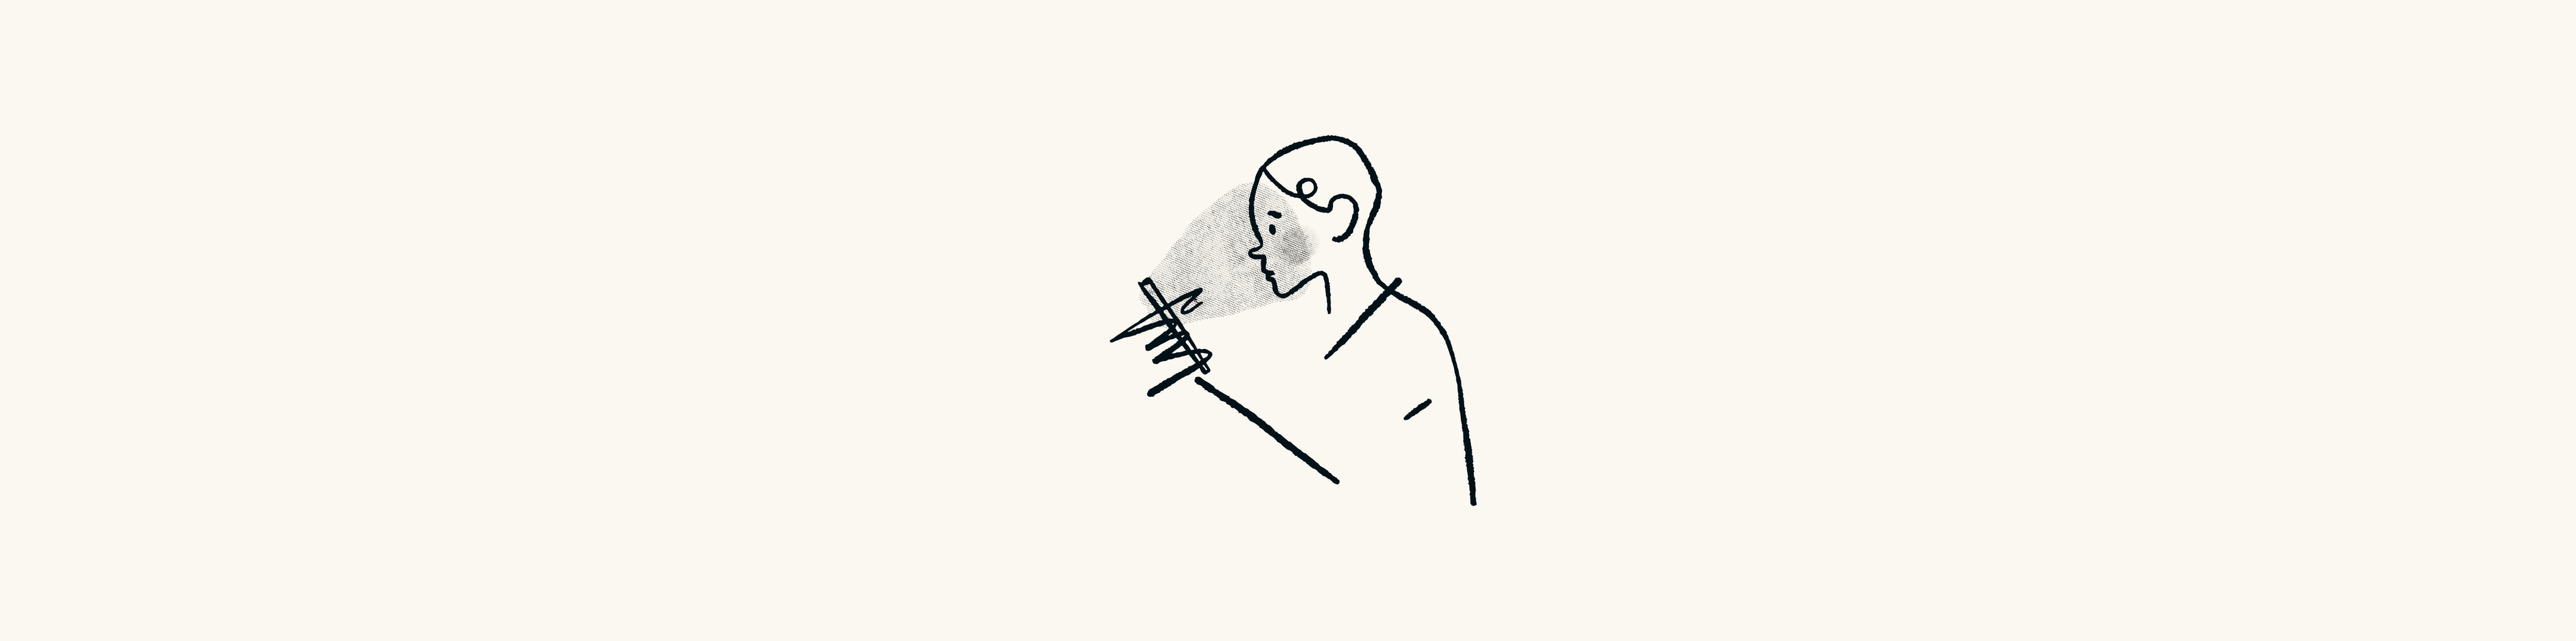
\includegraphics[width=\textwidth]{man_on_the_phone.png}
  %\caption{Find some picture related to the topic}
  \label{fig:teaser}
\end{teaserfigure}

\maketitle


\section{Introduction \& Motivation}

The aim of this project is to identify popular themes over time, starting from Tweets texts. The first step of the analysis consists in identifying popular topics on a specific day, but the focus of this work lies in finding themes that recur over time.

The problem that is faced falls within the large family of problems aimed at finding frequent items. More specifically, the data used belongs into the category of \textit{market-basket} model. In this kind of problems, there is on the one hand a set of \textit{items} and on the other \textit{baskets} containing them. A set of items present in many baskets is considered \textit{frequent}.

In the specific case of this project, dealing with social media texts, words are identified as items and tweets as baskets. By cleaning the text from noise (punctuation, extremely common words, ...) it is possible to identify common themes present in tweets. Once this is done, it's easy to investigate which topics are only momentarily popular and which are popular for longer periods of time.

Solving the problem is very relevant because it not only allows us to investigate what are the causes that make a topic popular, but also to predict the reaction of the public in the future. Furthermore, the solution algorithm can be extended to solve many other similar problems where the initial premises are the same.

The proposed solution exploits a Python optimized version of the \textit{APriori algorithm}, the most used in solving these problems. It is important to focus on the efficiency of the algorithm, as approaching the problem in a naïve way or trying to use brute-force could be very expensive in terms of time and resources.


%%%%%%%%%%%%%%%%%%%%%%%%%%%%%%%%

\section{Related work}

The APriori algorithm is at the core of the solution algorithm presented in this report. In the proposed solution, there is an initial need to identify frequent, day-to-day sets of words. APriori is used in this operation. The results provided will then be combined in order to achieve the predicted objective: find frequent topics over time. APriori and its functioning will be briefly explained below, given their importance.

APriori is among the most used algorithms to solve the problem of finding frequent itemsets. Frequent itemsets are a form of frequent pattern. Given examples that are sets of items and a minimum frequency, any set of items that occurs at least in the minimum number of examples is a frequent itemset \cite{Toivonen2010}. In the specific case considered, the goal is to identify the words (items) that are frequently used in many tweets (set of items).

At the hearth of the APriori algorithm there is a simple, yet powerful, premise: a large set of items cannot be frequent unless all the subsets that compose it are frequent. Following the logic of this principle, the algorithm initially focuses on smaller sets. In such manner, it manages to eliminate large sets of items from the list of candidates. This is crucial for the optimization of the solution.

%%%%%%%%%%%%%%%%%%%%%%%%%%%%%%%%

\section{Problem statement}\label{sect_probl_stat}

This section will specifically describe what input is required by the algorithm and what the generated output is.

\subsection*{Input}

The input required by the program is a dataset in \code{.pkl} format, necessary for the properties of the variables inside it to be maintained and recognized by the algorithm. There must be two columns in the dataset: \code{text} and \code{date}.

The \code{text} column contains texts of tweets. A tweet is defined as a sequence of words. For this reason, they are stored in the datasets as lists of words, or terms. Each term, or group of terms, is a potential frequent topic over time.

Every tweet must have an associated date. This is the purpose of the \code{date} column, which contains the information regard the day the tweet was posted, in the year-month-day format.

In order to fully understand the data used, it follows a small sample of the cleaned dataset used as input.

\begin{table}[h]
  \centering
  \begin{tabular}{@{}ll@{}}
  \toprule
  \textbf{date} & \textbf{text}                                         \\ \midrule
  2020-07-25    & {[}\textquotesingle smell\textquotesingle, \textquotesingle scent\textquotesingle, \textquotesingle hand\textquotesingle, \textquotesingle sanit\textquotesingle, \textquotesingle today\textquotesingle, ...{]} \\
  2020-08-29    & {[}\textquotesingle wear\textquotesingle, \textquotesingle cover\textquotesingle, \textquotesingle shop\textquotesingle, \textquotesingle includ\textquotesingle, \textquotesingle visit\textquotesingle, ...{]} \\
  ...           & ...                                                   \\ \bottomrule
  \end{tabular}
  \caption{Example of input data}
  \label{tab_input}
\end{table}

Notes: some words in Table \ref{tab_input} may appear truncated, other missing. It is intended, it will be explained in detail how the dataset was obtained in section \ref{sect_dataset}.

\subsection*{Output}

The interest is placed in finding groups of frequently repeated words within the tweets of several days, in order to find frequent topics over time. We assume that a group can also consist of a single word: even alone a word can identify a topic (for example \textit{mask}, or \textit{vaccine}).

Before proceeding with the output provided by the program, it is necessary to introduce the concept of \textbf{support}. It is a measure that allows to identify groups of frequent words based on a threshold value. The absolute support for an itemset $I$ is equal to the number of itemsets containing all items in $I$. Since there is a different number of tweets available for each day of the dataset, it is not feasible to use an absolute measure. For this reason it was used the absolute support divided by the total number of itemsets of the specific considered day. In practice, the support was found by dividing the total number of times in which a group of words appeared in a day by the total tweets of that day. 

It is possible for the user to decide the support value, when running the program. After numerous empirical tests, values around 0.015 are recommended. It is also possible to set the total number of results to be obtained, as well as the minimum number of days in which an itemset must be present to be part of the final solution.

After running the algorithm, a dataset is obtained as an output. It has the following columns:

\begin{itemize}
  \item \code{itemsets}, groups of frequent words stored as a frozenset;
  \item \code{dates}, the list of days in which the itemset was used;
  \item \code{supports}, the list of the supports, one for each day;
  \item \code{tot\_dates}, an absolute measure of the total days in which the itemset was found.
\end{itemize}

A sample of the output follows.

\begin{table}[h]
  \centering
  \small
  \tabcolsep=0.14cm
  \begin{tabular}{@{}llll@{}}
  \toprule
  \textbf{itemsets}         & \textbf{dates}                     & \textbf{supports}      & \textbf{tot\_dates}  \\ \midrule
  (pandemic)                & {[}2020-7-24, 2020-7-25, ...{]}    & {[}0.03, 0.05, ...{]}  & 26                   \\
  (covid, trump)            & {[}2020-7-24, 2020-8-16{]}         & {[}0.04, 0.07{]}       & 24                   \\
  (covid, india)          & {[}2020-7-25, 2020-7-26, ...{]}    & {[}0.03, 0.04, ...{]}  & 12                   \\
  ...                       & ...                                & ...                    & ...                  \\ \bottomrule
  \end{tabular}
  \caption{Example of output data}
\end{table}

%%%%%%%%%%%%%%%%%%%%%%%%%%%%%%%%

\section{Solution}\label{sect_solution}

In this section, the solution will be explained in detail.

\begin{itemize}
  \item The first step is to divide the tweets according to their publication day (column \code{date} of the dataset).

  \item The APriori algorithm is then applied to each subgroup, consisting of all the tweets of a given day. In this way, frequent itemsets are obtained for each day of the dataset.
  
  \item Finally, the last part of the algorithm associates to each itemset found the dates in which it is frequent, together with their support.
\end{itemize}

It is possible to find all the aforementioned steps in Figure \ref{figSol}.

\begin{figure}[h]
  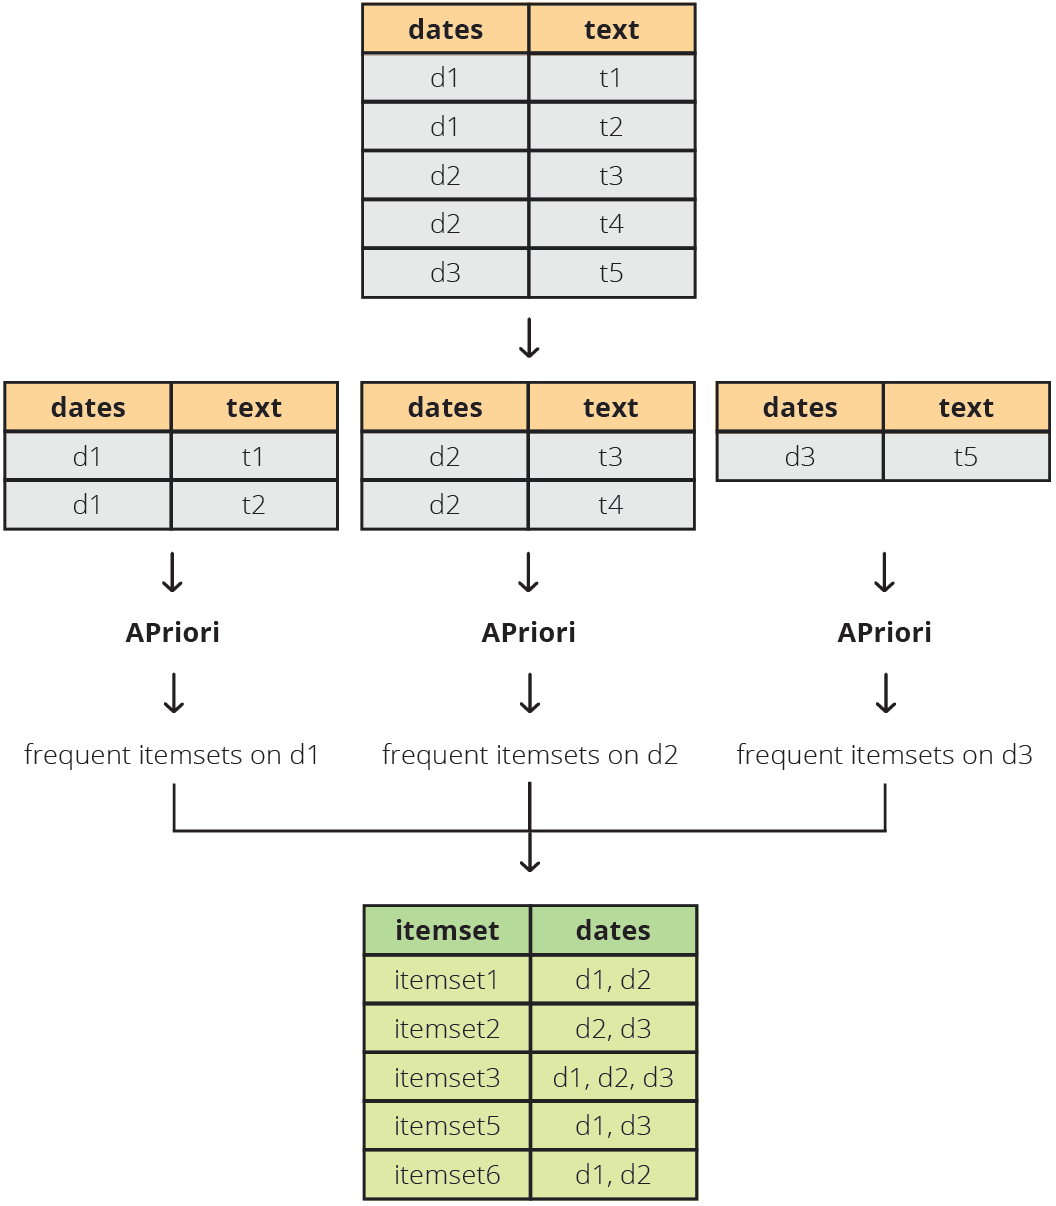
\includegraphics[scale=0.292]{solution.png}
  \centering
  \caption{graphical representation of the main steps of the algorithm}
  \label{figSol}
\end{figure} 

%%%%%%%%%%%%%%%%%%%%%%%%%%%%%%%%

\section{Implementation}
It follows a description of the tools used to implement the solution reported in section \ref{sect_solution}.

\subsection*{Programming language}
To solve the problem, the Python language was used (version 3.8.5). It was chosen for its very simple syntax rules, which facilitate code readability and program scalability.

\subsection*{Libraries}
To work properly, the algorithm needs some libraries, some already present in Python, others that need to be installed. For each of them, a brief explanation follows.

\vspace{2mm}
\code{pandas} As described in the official website, pandas is a fast, powerful, flexible and easy to use open source data analysis and manipulation tool, built on top of the Python programming language \cite{pandas}. Moreover, it offers data structures and operations for manipulating numeric tables and time series.

\vspace{2mm}
\code{datetime} Built-in Python module that supplies classes for manipulating dates and times.

\vspace{2mm}
\code{time} Built-in Python module which provides various time-related functions. It is not strictly related to the algorithm, but is used to track the time taken by the program to solve the problem and notify the user.

\vspace{2mm}
\code{sys} Built-in Python module that provides access to some variables used or maintained by the interpreter and to functions that interact strongly with the interpreter. It has been used to manage the parameters provided by the user, in order to provide a solution suited to his needs.

\vspace{2mm}
\code{mlxtend} It is a library of Python tools and extensions for data science. Their implementation of the APriori algorithm was used in the final solution algorithm.

\vspace{4mm}
Note: detailed information about Python core packages can be found on the official website \cite{python_website}. 

%%%%%%%%%%%%%%%%%%%%%%%%%%%%%%%%

\section{Dataset}\label{sect_dataset}

\subsection*{Original dataset}

The original dataset is public, it was created by Gabriel Preda and can be found on the Kaggle website \cite{kaggle_df}.

The author specifies that the tweets were obtained through the use of the Twitter API and a Python script. All tweets contain the hashtag \#covid19, and cover a period of time from July 24, 2020 to August 30, 2020. However, in some days the tweets were not collected. In figure \ref{dates_and_tweets} it is possible to see how many tweets have been gathered for each day. 

\begin{figure}[h]
  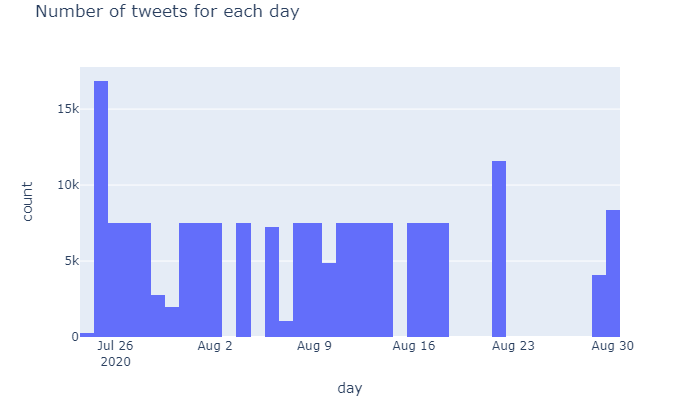
\includegraphics[scale=0.44]{dates_and_tweets.png}
  \centering
  \caption{number of tweets for each day}
  \label{dates_and_tweets}
\end{figure}

\subsection*{Column selection}

In addition to the texts of the tweets and the corresponding dates, the author has collected other variables, such as: 
\begin{itemize}
  \item \code{user\_location}
  \item \code{user\_name}
  \item \code{user\_description}
  \item \code{user\_created}
  \item \code{user\_followers}
  \item \code{user\_friends}
  \item \code{user\_favourites}
  \item \code{user\_verified}
  \item \code{source}
  \item \code{is\_retweet}
  \item \code{hashtags}
\end{itemize}

Since they are of no use to the study, they have been removed. As shown in section \ref{sect_probl_stat}, only the \code{text} and \code{date} columns have been preserved.

Column \code{date} contains information regarding the day and specific time the tweet was published. Only days were kept; information about the hours, minutes and seconds of the post were removed.

\subsection*{Text cleaning}

In the column \code{text}, the tweets texts are saved as a string. They are complete, therefore they contain punctuation, numbers, references to other users through the use of \code{@}, hashtags (and consequently the \code{\#} symbol), emojis, links, etc.

It is crucial to clean the texts so that they contain as much information as possible. To achieve this objective, various steps have been taken to clean the texts; they are reported below.

\subsubsection*{Lowercase text}
Each text was brought to its lowercase form, so that the algorithm does not differentiate words by capitalization.

\subsubsection*{Link removal}
Most tweets in the dataset are truncated. In these cases, the source link is shown at the end of the text, which adds no value to the text. Furthermore, users regularly post links that do not carry any information. For this reason all links have been removed.

\subsubsection*{Punctuation, symbols and numbers removal}
Initially it was decided to keep the numbers, but various tests showed that not only did they not carry information, but segmented it. As for punctuation and symbols, it is clear that in this case they are not useful, and so they have been removed.

\subsubsection*{Stopwords removal}
Stopwords are extremely common words, like prepositions, conjunctions and some of the most common verbs. They carry little value to the meaning of the sentences. For this reason, each word is checked and if it is considered a stopword, it is removed from the sentence. There is no single stopwords dictionary, in this analysis the one provided by the \code{nltk.corpus} library was used.

\subsubsection*{Stemming}
Stemming is the process of reducing inflected or derived words to their word base form. It was used because, intuitively, similar words can refer to the same topic (e.g., scared, scary, scariest, etc.). An example of stemming can be seen in Figure \ref{stem}.

\begin{figure}[h]
  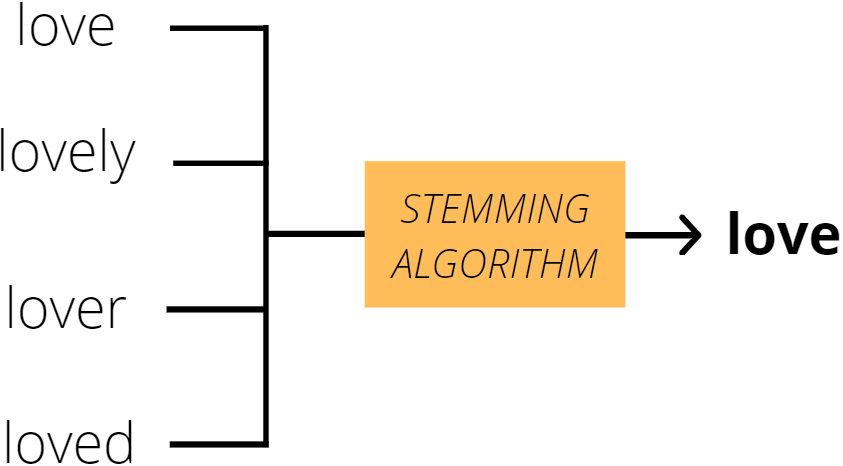
\includegraphics[scale=0.25]{stem.png}
  \centering
  \caption{simple example of stemming}
  \label{stem}
\end{figure}


In order to clean all the texts, about 180,000 iterations had to be done. The process was quite time consuming: it took about 3 hours on an Intel Core i7-9700K processor. For this reason, the final clean dataset has been saved, ready to be used as an input to the algorithm.

%%%%%%%%%%%%%%%%%%%%%%%%%%%%%%%%

\section{Experimental Evaluation}
 
Perform the necessary steps to illustrate that the method is good – or is not good. You can do this through a user evaluation and also through comparison with some base line method. It is up to you to select the base line method. Then you can compare the results and comment on what you observe. You should also care not only about the quality but also about the scalability, i.e., time, related to the size of the data. In this section, you should also have a subsection called Dataset in which you describe how you created the test dataset.

----------------------------------------------------------------------------

\subsection*{User evaluation}
In order to obtain a reasonable user evaluation, the algorithm code was sent to 10 people, along with instructions on how to execute it.

Five of these people are computer science graduates, thus they are accustomed to programming. None of them had problems running the code, despite using different operating systems (Windows, MacOS and Linux).

The other five are external to the world of information technology. Only one of them managed to successfully execute the code without external supervision. The problem others encountered was not with the instructions or execution of the specific code, but with the environment it requires to function properly. It was difficult for them to install the Python environment, manage environment variables and execute command line instructions. They needed outside supervision to be able to correctly run the code.

The best solution to make the code more accessible would be through the creation of an executable. Getting an executable from a \code{.py} file in Python is not straightforward, but there are some libraries that make the process easier. It is possible to use the \code{pyinstaller} library, although there are some limitations. The first one is that the generated executable only works on the same type of operating system on which it was created. So, to cover most of the users, an executable for Windows, Linux and MacOS should be generated. Furthermore, in this specific case, the user still has to run the program from the command line, if he wants to use custom parameters. After giving the executable to the four people who had been having problems installing Python, they were able to successfully run the program.

A further improvement would consist in adding a graphical interface, with the possibility to choose the parameters to be used in the execution of the algorithm, as well as the possibility to select the initial dataset and where to save the final results.

\subsection*{Time comparison with baseline}


\subsection*{Scalability evaluation}

%%
%% The next two lines define the bibliography style to be used, and the bibliography file.
\bibliographystyle{ACM-Reference-Format}
\bibliography{my_bibliography}

\end{document}
\endinput
